\chapter{Beschreibung des Versuchs}

\section{Versuchsaufbau}\label{Aufbau}

\begin{figure}[ht] 
  \centering
     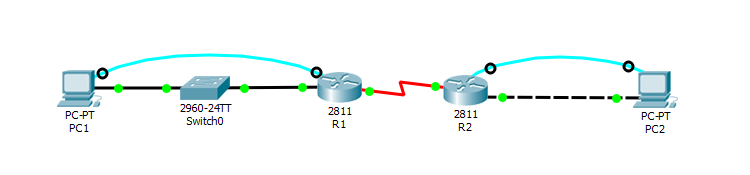
\includegraphics[width=\linewidth]{Graphics/Aufbau.PNG}
  \caption{Versuchsaufbau}
  \label{fig:aufbau}
\end{figure}

\subsection{Komponenten}

\begin{itemize}
  \item 2 Computer
  \begin{itemize}
    \item HyperTerminal als Emulationsprogramm
  \end{itemize}
  \item 2 Cisco 2811 Router
  \begin{itemize}
    \item Router 1: 
    \begin{itemize}
      \item Verbindung zu PC1 durch Konsolenkabel
      \item Verbindung zum Switch durch Straight-Through-Kabel
	\end{itemize}
	\item Router 2:
	\begin{itemize}
    \item Verbindung zu PC2 durch Crossover-Kabel und Konsolenkabel 
    \end{itemize}
    \item Verbindung untereinander durch Serial-Kabel
  \end{itemize}
  \item 1 Cisco 2960 Switch
  	\begin{itemize}
    	\item Verbindung zu PC1 durch Straight-Through-Kabel
   	\end{itemize}
\end{itemize}


\section{Versuchsdurchf�hrung}


\section{Versuchsziel}
